\documentclass[a4paper,12pt]{article}

%{
%  \usetheme{default}      
%  \usecolortheme{default}
%  \usefonttheme{default}  
%  \setbeamertemplate{navigation symbols}{}
%  \setbeamertemplate{caption}[numbered]
%  \setbeamertemplate{footline}[frame number]
%} 

\usepackage[english]{babel}
\usepackage[utf8x]{inputenc}
\usepackage{amsthm, amssymb, amsfonts, amsmath}
\usepackage{graphicx}
\usepackage{float}
\usepackage{lscape}
\usepackage{tikz}
\usetikzlibrary{calc,shapes}
\usepackage{mathtools}
\usepackage{mathrsfs}
\usepackage{tikz-cd}
\usetikzlibrary{positioning}
\usepackage{courier}
\usepackage{xcolor}
\usepackage{booktabs}
\usepackage{caption}
\usepackage[doublespacing]{setspace}
\usepackage{url}
\usepackage{subcaption}
%\pagestyle{empty} 		% This supresses the page numbers
\usepackage[authoryear]{natbib}
\usepackage{natbib} %Fundamental for good referencing, you also have to remember harvard.bst, for Harvard style refs.
\usepackage{hyperref}
\hypersetup{colorlinks=true, urlcolor=blue, linkcolor=blue, citecolor=blue}

\newcommand{\comment}[1]{{\color{red}#1}}

\newcommand{\rot}[2]{\rule{1em}{0pt}%
\makebox[0cm][c]{\rotatebox{#1}{\ #2}}}
\newcommand{\sym}[1]{\rlap{#1}}

\usepackage{siunitx} % centering in tables
	\sisetup{
		detect-mode,
		tight-spacing		= true,
		group-digits		= false ,
		input-signs		= ,
		input-symbols		= ( ) [ ] - + *,
		input-open-uncertainty	= ,
		input-close-uncertainty	= ,
		table-align-text-post	= false
        }

\newcolumntype{$}{>{\global\let\currentrowstyle\relax}}
\newcolumntype{^}{>{\currentrowstyle}}
\newcommand{\rowstyle}[1]{\gdef\currentrowstyle{#1}%
  #1\ignorespaces
}
%$

\usepackage{geometry}
	\geometry{
	a4paper,
	total={170mm,257mm},
	left=25mm,
	right=25mm,
	top=25mm,
	bottom=25mm
}

%%%%%%%%%%%%%%%%%%%%%%%%%%%%%%%%%%%%%%%%%%%%%%%%%%%%%%%%%%%%%%%%%%%%%%%%%%%%%%%%%%%%
%%%%%%%%%%%%%%%%%%%%%%%%%%%%%%%%%%%%%%%%%%%%%%%%%%%%%%%%%%%%%%%%%%%%%%%%%%%%%%%%%%%%

\begin{document}

\textbf{Test scores and month of birth}
\bigskip \bigskip

\vspace{3mm}

\begin{figure}[H]
\centering
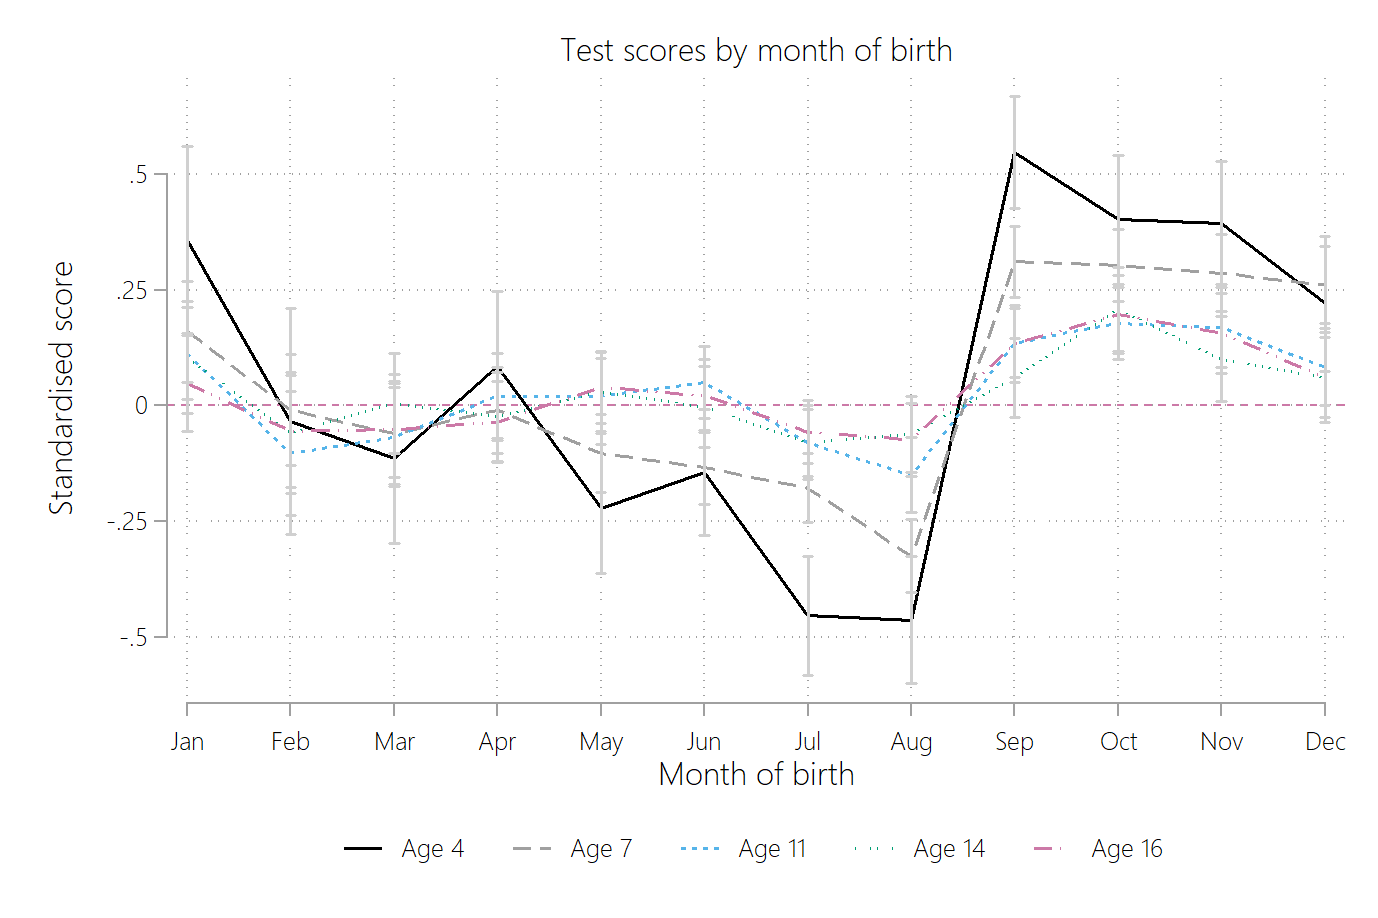
\includegraphics[width=0.8\linewidth]{../figures/MoB.png}
\caption{Standardised test scores at different ages by month of birth.}
\end{figure}

\begin{figure}[H]
\centering \label{fig:MoBnew}
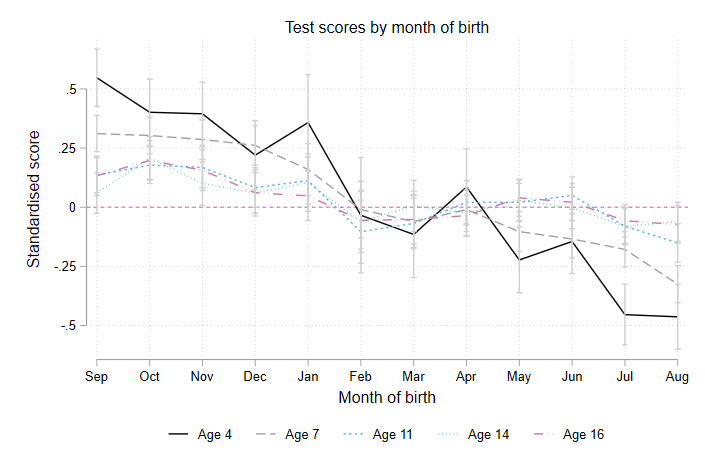
\includegraphics[width=0.8\linewidth]{../figures/MoBnew.png}
\caption{Standardised test scores at different ages by month of birth - showing approx linear trend.}
\end{figure}
\clearpage

\begin{equation*} 
Y_i = \sum_{m=1}^{11} \beta_m MoB_{m} + \lambda PGS_i + \alpha female_i + \sum_{k=1}^{10} \phi_k PC_k + u_i
\end{equation*} 

where $Y_{i}$ is standardised test score of individual $i$, and $\beta_m$ are the 11 month-specific coefficients ($1=Sep, 2=Oct, ..., 11=Jul$, as in \autoref{fig:MoBnew}). We control for the child's EA polygenic score, standardized to have mean 0 and std dev 1. Also control for gender and the first 10 principal components.

\bigskip \bigskip 

\begin{table}[H]
\caption{OLS of test scores on MoB (dummies)}
\centering
{\footnotesize
\begin{tabular}{lcccccccccccccc}
\toprule
            &\multicolumn{1}{c}{(1)}&\multicolumn{1}{c}{(2)}&\multicolumn{1}{c}{(3)}&\multicolumn{1}{c}{(4)}&\multicolumn{1}{c}{(5)}\\
            &\multicolumn{1}{c}{Age 4}&\multicolumn{1}{c}{Age 7}&\multicolumn{1}{c}{Age 11}&\multicolumn{1}{c}{Age 14}&\multicolumn{1}{c}{Age 16}\\
\midrule
Oct         &      -0.141\sym{***}&      -0.036\sym{***}&       0.025\sym{***}&       0.111\sym{***}&       0.063\sym{***}\\
            &     (0.005)         &     (0.001)         &     (0.002)         &     (0.002)         &     (0.002)         \\
\addlinespace
Nov         &      -0.168\sym{***}&      -0.045\sym{***}&       0.022\sym{***}&       0.030\sym{***}&       0.038\sym{***}\\
            &     (0.008)         &     (0.002)         &     (0.002)         &     (0.002)         &     (0.002)         \\
\addlinespace
Dec         &      -0.310\sym{***}&      -0.070\sym{***}&      -0.042\sym{***}&      -0.001         &       0.003\sym{*}  \\
            &     (0.004)         &     (0.002)         &     (0.003)         &     (0.002)         &     (0.002)         \\
\addlinespace
Jan         &      -0.207\sym{***}&      -0.186\sym{***}&      -0.038\sym{***}&       0.005\sym{**} &       0.049\sym{***}\\
            &     (0.005)         &     (0.003)         &     (0.003)         &     (0.002)         &     (0.002)         \\
\addlinespace
Feb         &      -0.575\sym{***}&      -0.317\sym{***}&      -0.235\sym{***}&      -0.120\sym{***}&      -0.092\sym{***}\\
            &     (0.006)         &     (0.003)         &     (0.001)         &     (0.003)         &     (0.002)         \\
\addlinespace
Mar         &      -0.611\sym{***}&      -0.382\sym{***}&      -0.208\sym{***}&      -0.064\sym{***}&      -0.150\sym{***}\\
            &     (0.009)         &     (0.002)         &     (0.002)         &     (0.002)         &     (0.001)         \\
\addlinespace
Apr         &      -0.445\sym{***}&      -0.349\sym{***}&      -0.133\sym{***}&      -0.115\sym{***}&      -0.086\sym{***}\\
            &     (0.009)         &     (0.001)         &     (0.002)         &     (0.002)         &     (0.002)         \\
\addlinespace
May         &      -0.743\sym{***}&      -0.460\sym{***}&      -0.157\sym{***}&      -0.075\sym{***}&       0.012\sym{***}\\
            &     (0.006)         &     (0.002)         &     (0.003)         &     (0.003)         &     (0.002)         \\
\addlinespace
Jun         &      -0.681\sym{***}&      -0.462\sym{***}&      -0.103\sym{***}&      -0.085\sym{***}&      -0.087\sym{***}\\
            &     (0.006)         &     (0.002)         &     (0.002)         &     (0.002)         &     (0.002)         \\
\addlinespace
Jul         &      -1.003\sym{***}&      -0.522\sym{***}&      -0.242\sym{***}&      -0.169\sym{***}&      -0.117\sym{***}\\
            &     (0.007)         &     (0.002)         &     (0.003)         &     (0.002)         &     (0.002)         \\
\addlinespace
Aug         &      -0.972\sym{***}&      -0.654\sym{***}&      -0.302\sym{***}&      -0.146\sym{***}&      -0.130\sym{***}\\
            &     (0.008)         &     (0.002)         &     (0.003)         &     (0.001)         &     (0.002)         \\
\addlinespace
PGS         &       0.135\sym{***}&       0.244\sym{***}&       0.309\sym{***}&       0.311\sym{***}&       0.121\sym{***}\\
            &     (0.026)         &     (0.009)         &     (0.012)         &     (0.010)         &     (0.012)         \\
\midrule
R2          &       0.187         &       0.138         &       0.113         &       0.110         &       0.035         \\
Observations&        1826         &        5734         &        6075         &        5240         &        7268         \\

\bottomrule
\addlinespace[.75ex]
\end{tabular}
\caption*{\scriptsize{Robust standard errors clustered by MoB in parentheses. * $p < 0.1$, ** $p < 0.05$, *** $p < 0.01$.}}
}
\end{table}


To allow for linear trend in MoB, i.e.:
\begin{equation*} 
Y_i = \beta MoB + \lambda PGS_i + \alpha female_i + \sum_{k=1}^{10} \phi_k PC_k + u_i
\end{equation*} 

where $MoB$ is coded as $1=Sep, 2=Oct, \ldots, 11=Jul$. This gives the following estimates:

\bigskip \bigskip

\begin{table}[H]
\caption{OLS of test scores on MoB (linear)}
\centering
{\footnotesize
\begin{tabular}{lcccccccccccccc}
\toprule
            &\multicolumn{1}{c}{(1)}&\multicolumn{1}{c}{(2)}&\multicolumn{1}{c}{(3)}&\multicolumn{1}{c}{(4)}&\multicolumn{1}{c}{(5)}\\
            &\multicolumn{1}{c}{Age 4}&\multicolumn{1}{c}{Age 7}&\multicolumn{1}{c}{Age 11}&\multicolumn{1}{c}{Age 14}&\multicolumn{1}{c}{Age 16}\\
\midrule
Treated     &       0.684\sym{***}&       0.451\sym{***}&       0.186\sym{***}&       0.142\sym{***}&       0.112\sym{***}\\
            &     (0.084)         &     (0.035)         &     (0.041)         &     (0.028)         &     (0.027)         \\
\addlinespace
Treated*MoB &       0.117\sym{***}&       0.076\sym{***}&       0.038\sym{**} &       0.026\sym{***}&       0.011         \\
            &     (0.029)         &     (0.013)         &     (0.016)         &     (0.008)         &     (0.013)         \\
\addlinespace
MoB         &      -0.101\sym{***}&      -0.057\sym{***}&      -0.026\sym{*}  &      -0.017\sym{***}&      -0.007         \\
            &     (0.024)         &     (0.011)         &     (0.013)         &     (0.005)         &     (0.011)         \\
\addlinespace
PGS         &       0.136\sym{***}&       0.244\sym{***}&       0.309\sym{***}&       0.312\sym{***}&       0.121\sym{***}\\
            &     (0.025)         &     (0.009)         &     (0.012)         &     (0.011)         &     (0.012)         \\
\midrule
R2          &       0.171         &       0.136         &       0.110         &       0.108         &       0.033         \\
Observations&        1826         &        5734         &        6075         &        5240         &        7268         \\

\bottomrule
\addlinespace[.75ex]
\end{tabular}
\caption*{\scriptsize{Robust standard errors clustered by MoB in parentheses. * $p < 0.1$, ** $p < 0.05$, *** $p < 0.01$.}}
}
\end{table}


Note that the $R^2$ is much lower for the KS4 specification (column 5). Not sure why this is. The KS4 variable is measured slightly differently, but should still pick up EA. Would have to look into this more if we want to go ahead with this, or let's just focus on Age 4--14 for now.

I prefer this second specification with linear MoB. I think this model would be preferred statistically too, e.g. very similar R2 using fewer df.


\clearpage
Next, we run the following regression, allowing for an interaction between G and E:

\begin{equation*} 
Y_i =  \sum_{m=1}^{11} \eta_m MoB_{m} \times PGS_i + \sum_{m=1}^{11} \beta_m MoB_{m} + \lambda PGS_i + \alpha female_i + \sum_{k=1}^{10} \phi_k PC_k + u_i
\end{equation*} 



\begin{table}[H]
\caption{OLS of test scores on MoB (dummies) and interactions with PGS}
\centering
{\tiny
\begin{tabular}{lcccccccccccccc}
\toprule
            &\multicolumn{1}{c}{(1)}&\multicolumn{1}{c}{(2)}&\multicolumn{1}{c}{(3)}&\multicolumn{1}{c}{(4)}&\multicolumn{1}{c}{(5)}\\
            &\multicolumn{1}{c}{Age 4}&\multicolumn{1}{c}{Age 7}&\multicolumn{1}{c}{Age 11}&\multicolumn{1}{c}{Age 14}&\multicolumn{1}{c}{Age 16}\\
\midrule
Oct*PGS     &       0.116\sym{***}&       0.055\sym{***}&      -0.011\sym{***}&       0.064\sym{***}&       0.030\sym{***}\\
            &     (0.008)         &     (0.004)         &     (0.002)         &     (0.003)         &     (0.003)         \\
\addlinespace
Nov*PGS     &       0.144\sym{***}&       0.059\sym{***}&       0.054\sym{***}&       0.090\sym{***}&       0.037\sym{***}\\
            &     (0.006)         &     (0.003)         &     (0.003)         &     (0.003)         &     (0.002)         \\
\addlinespace
Dec*PGS     &       0.087\sym{***}&       0.038\sym{***}&       0.044\sym{***}&       0.032\sym{***}&      -0.032\sym{***}\\
            &     (0.007)         &     (0.002)         &     (0.002)         &     (0.002)         &     (0.002)         \\
\addlinespace
Jan*PGS     &       0.050\sym{***}&      -0.020\sym{***}&      -0.055\sym{***}&       0.024\sym{***}&      -0.028\sym{***}\\
            &     (0.011)         &     (0.002)         &     (0.002)         &     (0.002)         &     (0.002)         \\
\addlinespace
Feb*PGS     &       0.224\sym{***}&       0.052\sym{***}&       0.105\sym{***}&       0.077\sym{***}&       0.008\sym{***}\\
            &     (0.008)         &     (0.003)         &     (0.003)         &     (0.003)         &     (0.003)         \\
\addlinespace
Mar*PGS     &      -0.103\sym{***}&       0.100\sym{***}&       0.126\sym{***}&      -0.013\sym{***}&       0.045\sym{***}\\
            &     (0.006)         &     (0.002)         &     (0.002)         &     (0.004)         &     (0.002)         \\
\addlinespace
Apr*PGS     &      -0.004         &       0.049\sym{***}&       0.017\sym{***}&       0.001         &       0.020\sym{***}\\
            &     (0.009)         &     (0.005)         &     (0.003)         &     (0.003)         &     (0.004)         \\
\addlinespace
May*PGS     &       0.084\sym{***}&       0.089\sym{***}&       0.076\sym{***}&       0.031\sym{***}&       0.088\sym{***}\\
            &     (0.007)         &     (0.003)         &     (0.002)         &     (0.003)         &     (0.002)         \\
\addlinespace
Jun*PGS     &       0.233\sym{***}&       0.020\sym{***}&       0.010\sym{***}&      -0.025\sym{***}&      -0.068\sym{***}\\
            &     (0.004)         &     (0.002)         &     (0.002)         &     (0.002)         &     (0.002)         \\
\addlinespace
Jul*PGS     &       0.172\sym{***}&       0.054\sym{***}&      -0.019\sym{***}&       0.018\sym{***}&       0.013\sym{***}\\
            &     (0.008)         &     (0.003)         &     (0.002)         &     (0.003)         &     (0.003)         \\
\addlinespace
Aug*PGS     &       0.053\sym{***}&       0.064\sym{***}&       0.022\sym{***}&       0.043\sym{***}&       0.007\sym{**} \\
            &     (0.002)         &     (0.003)         &     (0.003)         &     (0.003)         &     (0.003)         \\
\addlinespace
Oct         &      -0.132\sym{***}&      -0.031\sym{***}&       0.027\sym{***}&       0.112\sym{***}&       0.062\sym{***}\\
            &     (0.005)         &     (0.001)         &     (0.001)         &     (0.002)         &     (0.002)         \\
\addlinespace
Nov         &      -0.163\sym{***}&      -0.040\sym{***}&       0.023\sym{***}&       0.036\sym{***}&       0.038\sym{***}\\
            &     (0.008)         &     (0.002)         &     (0.002)         &     (0.002)         &     (0.002)         \\
\addlinespace
Dec         &      -0.303\sym{***}&      -0.065\sym{***}&      -0.040\sym{***}&       0.001         &       0.003\sym{*}  \\
            &     (0.004)         &     (0.002)         &     (0.003)         &     (0.002)         &     (0.001)         \\
\addlinespace
Jan         &      -0.203\sym{***}&      -0.183\sym{***}&      -0.039\sym{***}&       0.008\sym{**} &       0.049\sym{***}\\
            &     (0.006)         &     (0.003)         &     (0.003)         &     (0.002)         &     (0.002)         \\
\addlinespace
Feb         &      -0.543\sym{***}&      -0.312\sym{***}&      -0.232\sym{***}&      -0.114\sym{***}&      -0.092\sym{***}\\
            &     (0.006)         &     (0.003)         &     (0.001)         &     (0.003)         &     (0.002)         \\
\addlinespace
Mar         &      -0.644\sym{***}&      -0.374\sym{***}&      -0.205\sym{***}&      -0.064\sym{***}&      -0.148\sym{***}\\
            &     (0.009)         &     (0.002)         &     (0.002)         &     (0.002)         &     (0.001)         \\
\addlinespace
Apr         &      -0.444\sym{***}&      -0.344\sym{***}&      -0.132\sym{***}&      -0.113\sym{***}&      -0.086\sym{***}\\
            &     (0.009)         &     (0.001)         &     (0.002)         &     (0.002)         &     (0.002)         \\
\addlinespace
May         &      -0.737\sym{***}&      -0.457\sym{***}&      -0.160\sym{***}&      -0.072\sym{***}&       0.008\sym{***}\\
            &     (0.006)         &     (0.002)         &     (0.002)         &     (0.002)         &     (0.002)         \\
\addlinespace
Jun         &      -0.670\sym{***}&      -0.458\sym{***}&      -0.102\sym{***}&      -0.084\sym{***}&      -0.083\sym{***}\\
            &     (0.006)         &     (0.002)         &     (0.002)         &     (0.002)         &     (0.002)         \\
\addlinespace
Jul         &      -1.002\sym{***}&      -0.518\sym{***}&      -0.239\sym{***}&      -0.167\sym{***}&      -0.117\sym{***}\\
            &     (0.006)         &     (0.001)         &     (0.002)         &     (0.002)         &     (0.001)         \\
\addlinespace
Aug         &      -0.970\sym{***}&      -0.649\sym{***}&      -0.301\sym{***}&      -0.144\sym{***}&      -0.129\sym{***}\\
            &     (0.008)         &     (0.002)         &     (0.003)         &     (0.002)         &     (0.002)         \\
\addlinespace
PGS         &       0.043\sym{***}&       0.197\sym{***}&       0.282\sym{***}&       0.283\sym{***}&       0.110\sym{***}\\
            &     (0.005)         &     (0.002)         &     (0.002)         &     (0.002)         &     (0.001)         \\
\midrule
R2          &       0.194         &       0.139         &       0.115         &       0.111         &       0.037         \\
Observations&        1826         &        5734         &        6075         &        5240         &        7268         \\

\bottomrule
\addlinespace[.75ex]
\end{tabular}
\caption*{\scriptsize{Robust standard errors clustered by MoB in parentheses. * $p < 0.1$, ** $p < 0.05$, *** $p < 0.01$.}}
}
\end{table}

I don't think this is very informative. Some are positive, others negative, which would suggest that in some months having a high PGS increases inequalities in EA between Aug and Sept births, but it reduces inequalities in other months. It also doesn't seem particularly robust across specifications. Therefore, allowing for a linear trend in MoB:

\bigskip \bigskip

\begin{table}[H]
\caption{OLS of test scores on MoB (linear) and interactions with PGS}
\centering
{\footnotesize
\begin{tabular}{lcccccccccccccc}
\toprule
            &\multicolumn{1}{c}{(1)}&\multicolumn{1}{c}{(2)}&\multicolumn{1}{c}{(3)}&\multicolumn{1}{c}{(4)}&\multicolumn{1}{c}{(5)}\\
            &\multicolumn{1}{c}{Age 4}&\multicolumn{1}{c}{Age 7}&\multicolumn{1}{c}{Age 11}&\multicolumn{1}{c}{Age 14}&\multicolumn{1}{c}{Age 16}\\
\midrule
Treated     &       0.682\sym{***}&       0.450\sym{***}&       0.185\sym{***}&       0.142\sym{***}&       0.140\sym{***}\\
            &     (0.083)         &     (0.034)         &     (0.041)         &     (0.028)         &     (0.026)         \\
\addlinespace
Treated*PGS &      -0.019         &      -0.025         &       0.009         &       0.028         &       0.007         \\
            &     (0.066)         &     (0.021)         &     (0.028)         &     (0.021)         &     (0.024)         \\
\addlinespace
Treated*MoB &       0.112\sym{***}&       0.077\sym{***}&       0.038\sym{**} &       0.026\sym{***}&       0.022\sym{**} \\
            &     (0.030)         &     (0.012)         &     (0.016)         &     (0.007)         &     (0.008)         \\
\addlinespace
MoB*PGS     &       0.029         &      -0.005         &      -0.019\sym{*}  &       0.008\sym{**} &      -0.004         \\
            &     (0.020)         &     (0.004)         &     (0.009)         &     (0.003)         &     (0.006)         \\
\addlinespace
MoB*PGS*Treated&      -0.032         &       0.009         &       0.021\sym{*}  &      -0.006         &       0.003         \\
            &     (0.021)         &     (0.006)         &     (0.011)         &     (0.004)         &     (0.006)         \\
\addlinespace
MoB         &      -0.097\sym{***}&      -0.057\sym{***}&      -0.026\sym{*}  &      -0.017\sym{***}&      -0.010         \\
            &     (0.025)         &     (0.011)         &     (0.013)         &     (0.005)         &     (0.007)         \\
\addlinespace
PGS         &       0.178\sym{**} &       0.219\sym{***}&       0.278\sym{***}&       0.297\sym{***}&       0.277\sym{***}\\
            &     (0.069)         &     (0.017)         &     (0.018)         &     (0.016)         &     (0.023)         \\
\midrule
R2          &       0.179         &       0.139         &       0.111         &       0.111         &       0.115         \\
Observations&        1826         &        5734         &        6075         &        5240         &        6069         \\

\bottomrule
\addlinespace[.75ex]
\end{tabular}
\caption*{\scriptsize{Robust standard errors clustered by MoB in parentheses. * $p < 0.1$, ** $p < 0.05$, *** $p < 0.01$.}}
}
\end{table}


hmmm... bit of a shame really! But a null-result is also a result... We haven't controlled for the school and cohort fixed effects yet.


\end{document}

%----------------------------------------------------------------------------------%
\footnotesize
%\bibliographystyle{chicago}
\onehalfspacing
%\bibliography{References}

%----------------------------------------------------------------------------------%


\end{document}





